\documentclass{scrreprt}

\usepackage{graphicx}
\usepackage{tikz}
\usepackage{amstext}
\usepackage{hyperref}
\usepackage{amsfonts}
\usepackage{tabularx}
\usepackage{multirow}
\usepackage{amssymb}
\usepackage{textcomp}
\usepackage[left=2.5cm, right=2.5cm, top=2cm, bottom=2cm]{geometry}
\newcommand\tab[1][1cm]{\hspace*{#1}}

\usepackage{listings}
\usepackage{color}

\definecolor{dkgreen}{rgb}{0,0.6,0}
\definecolor{gray}{rgb}{0.5,0.5,0.5}
\definecolor{mauve}{rgb}{0.58,0,0.82}

\lstset{frame=tb,
  language=Java,
  aboveskip=3mm,
  belowskip=3mm,
  showstringspaces=false,
  columns=flexible,
  basicstyle={\small\ttfamily},
  numbers=none,
  numberstyle=\tiny\color{gray},
  keywordstyle=\color{blue},
  commentstyle=\color{dkgreen},
  stringstyle=\color{mauve},
  breaklines=true,
  breakatwhitespace=true,
  tabsize=3
}

\hypersetup{
  colorlinks=false,
  linkbordercolor=blue,
  pdfborderstyle={/S/U/W 0}
}
\title{\textbf{Algorithmen und Datenstrukturen}}
\author{\href{https://github.com/bircni}{\color{blue}github/bircni}}
%\date{\href{https://ko-fi.com/toiletcoders}{\color{black}little donation}}
\begin{document}
\pagenumbering{gobble}
\maketitle
\pagebreak
\renewcommand{\contentsname}{Inhaltsverzeichnis}
%\renewcommand{\cftdot}{}
\setcounter{tocdepth}{1}
\tableofcontents
\addtocontents{toc}{~\hfill\textbf{Seite}\par}
\pagebreak
%\pagenumbering{arabic}
\chapter{Mathematische Grundlagen}
\section{Reihen}
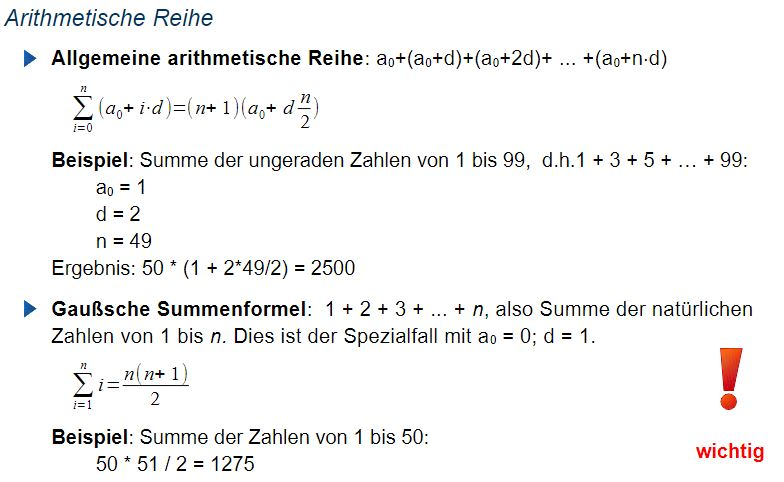
\includegraphics[width=0.65\textwidth]{graphics/reihen-arithmetisch}
\section{Potenzen und Logarithmen}
Der Logarithmus ist die Inverse der Potenzfunktion. $\log_a(x) = y \quad \Longleftrightarrow  \quad a^y = x$
\\\textbf{spezielle Logarithmen:}
\\$ld(x)=log_2(x)$, $lg(x)=log_10(x)$, $ln(x)=log_e(x)$
\section{Notationskonventionen}
$\lceil x \rceil$ zur nächsten ganzen Zahl aufrunden
\\$\lfloor x \rfloor$ zur nächsten ganzen Zahl abrunden
\\$[a .. b] = {x \arrowvert a \leq x \wedge x \leq b}$ mit Intervallgrenzen
\\$]a .. b[ = {x \arrowvert a < x \wedge x < b}$ ohne Intervallgrenzen
\\$arr[i .. k]$ Teilfolge der Elemente von $arr[i]$ bis $arr[k]$
\section{Grundbegriffe der Graphentheorie}
Graphen bestehen aus einer Menge von Knoten und Kanten, die diese verbinden.
\\Ein Graph ist gerichtet, wenn die Kanten eine Richtung haben.
\\Für einen Knoten v eines gerichteten Graphen $G=(V,E)$ ist der Eingangsgrad $indeg(v)$ die Anzahl der Kanten,
die in v enden, und der Ausgangsgrad $outdeg(v)$ die Anzahl der Kanten, die von v ausgehen.
\\Ein Zyklus ist ein Weg der bei einem Knoten startet und endet.
\\Ein gerichteter Graph ist zusammenhängend, wenn es einen Weg zwischen jedem Knotenpaar gibt.
\\Ein Baum hat einen Knoten als Wurzel, jeder Knoten hat genau einen Vorgänger und ist zusammenhängend.
\\Ein Knoten ohne Kinder heißt Blatt. Ein leerer Baum hat die Höhe 0.
Ein Binärbaum ist ein Baum, dessen Knoten maximal zwei Kinder haben.
\\Traversierungen: Preorder (WLR), Inorder (LWR), Postorder (LRW)
\chapter{Rekursive Algorithmen}
\section{Prinzip der Rekursion}
Ein rekursiver Algorithmus besteht aus einem Basisfall und einem rekursiven Aufruf.
\\Der rekursive Aufruf muss immer kleiner werden, damit die Rekursion endet.
\\Die Rekursion kann durch eine Schleife ersetzt werden.
\begin{lstlisting}
  public static double sum_v2(double[] arr) {
  return sum_v2(arr, 0, arr.length-1);
  }
/** Berechnet Summe der Werte von arr[firstIndex..lastIndex] */
  private static double sum_v2(double[] arr, int firstIndex,int lastIndex) {
  if (firstIndex == lastIndex) {
    // zu summierender Bereich besteht nur aus einem Element
    return arr[firstIndex];
  }
  else {
    int mid = (firstIndex + lastIndex) / 2;
    return sum_v2(arr, firstIndex, mid) + sum_v2(arr, mid+1, lastIndex);
  }}
  \end{lstlisting}
\section{Korrektheit rekursiver Algorithmen}
Ein Beweisverfahren ist die Berechnungsinduktion.
\\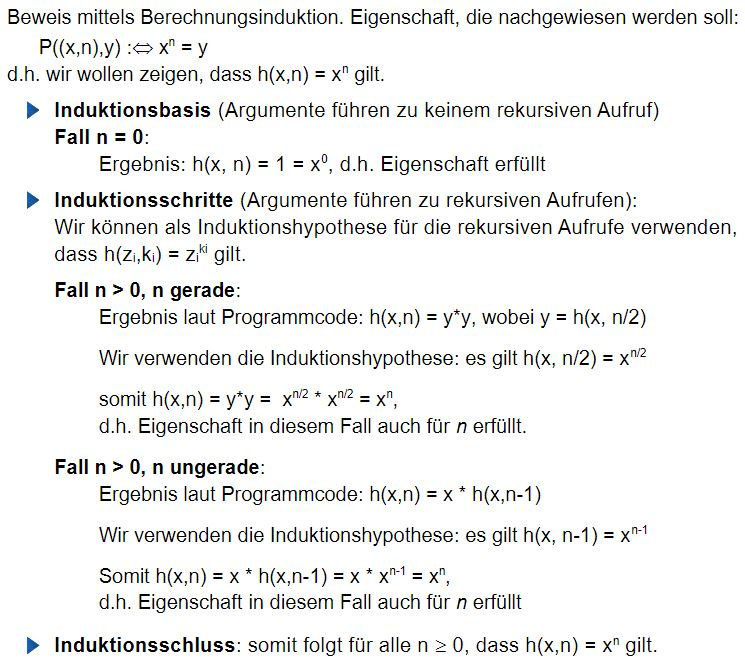
\includegraphics[width=0.65\textwidth]{graphics/3-2Korrektheit}
%4:
\end{document}